\documentclass[a4paper,12pt]{article}
\usepackage[left=2cm,top=1.7cm,bottom=2cm,right=2cm]{geometry}
\usepackage{fancyhdr}
\usepackage{graphicx}
\usepackage[utf8]{inputenc}


\title{Design Analysis}
\author{Group Project 3 - Group 2}
\date{March 21 2008}

\begin{document}
\maketitle
\newpage
\tableofcontents
\newpage



\section{Introduction}
This class diagram highlights the classes discovered during the analysis,
and some additional classes discovered during the design of our application.
You will notice that there are no methods in our classes related to the reading, the creation, the deletion nor the updating.
There are no such methods because we assume that these features are handled from the roots by the Grails Framework.

\section{Class diagram}
\begin{figure}[htbp]
\begin{center}
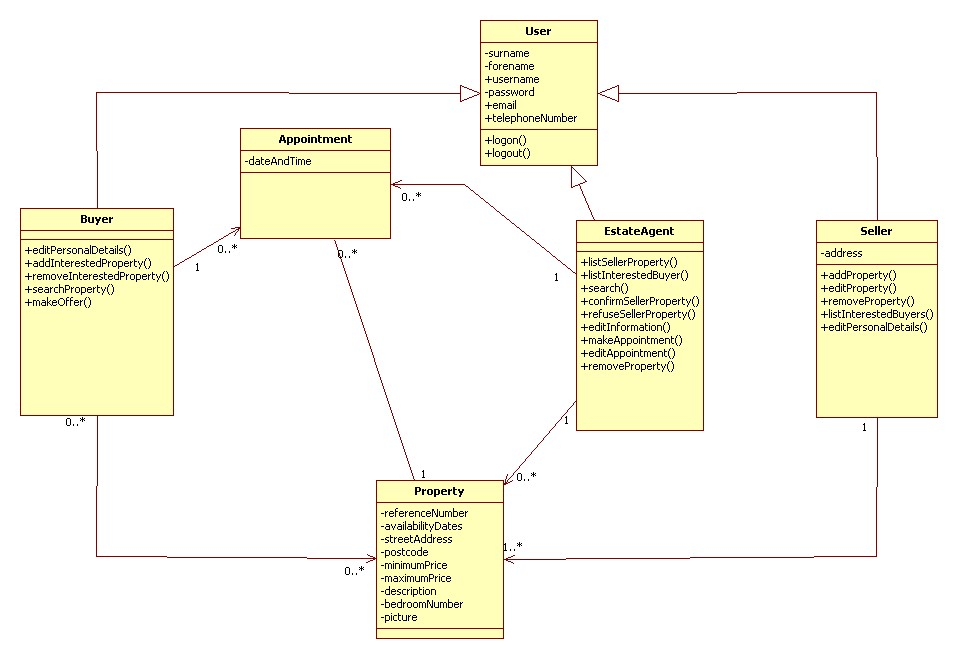
\includegraphics[width=\linewidth]{pics/classDiagram.jpg}
\end{center}
\caption{\footnotesize Class Diagram of Napier Estate Agency}
\end{figure}
\subsection {Classes description}

\subsubsection{EstateAgent class}
An estate agent inherits from a User.
He can :
\begin{itemize}
\item List his properties
\item List the buyers interested in his properties
\item Search for a property
\item Validate (or not) a property in order to make it available on the website.
\item Edit the details of a property
\item Edit an appointment
\item Remove a property
\end{itemize}

\subsubsection{Buyer class}
A buyer inherits from a User.
He can :
\begin{itemize}
\item Add a property to his interested list
\item Remove a property from this list
\item Search for a property
\item Set up an appointment
\item Make an offer for a property
\end{itemize}

\subsubsection{Seller class}
A seller inherits from a User.
He can :
\begin{itemize}
\item Add his property to the website (which is going to be validated by an estate agent)
\item See the list of buyers interested in his properties
\end{itemize}

\subsubsection{User class}
The Seller class, the Buyer class and the EstateAgent class have some common attributes and behaviours,
that's why a parent class, User, has been created to generalise theses attributes and behaviours.
A user is characterised by :
\begin{itemize}
\item His surname
\item His forename
\item A password
\item An email
\item His telephone number (should be formatted like a UK number)
\end{itemize}
This class also handles the login and the logout of a user.

\subsubsection{Property class}
This class describes a property. A property is characterised by:
\begin{itemize}
\item A reference number (unique identifier for a property)
\item A set of availability dates
\item A postcode (constrained by the UK Postcode format)
\item A minimum price
\item A maximum price
\item A short description of the property
\item The number of bedrooms
\item A set of images
\end{itemize}

\subsubsection{Appointment class}
This class describes an appointment, which is created with a particular date and a particular time.
Constraint: An estate agent or a buyer can't have more than one appointment on the same date.



\section{Use-Case Diagram}

\subsection{Napier Estate Agency use case diagram}
\begin{figure}[htbp]
\begin{center}
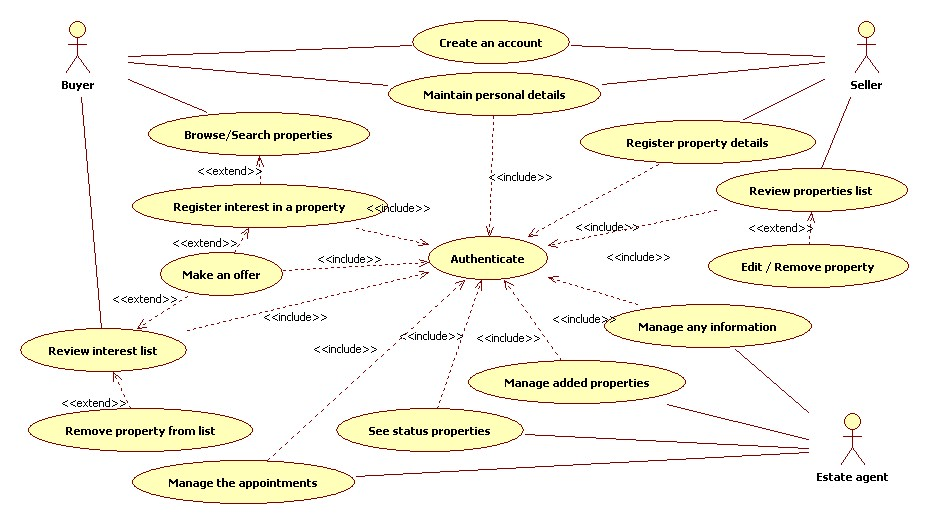
\includegraphics[width=\linewidth]{pics/useCases.jpg}
\end{center}
\caption{\footnotesize Use-Case Diagram of Napier Estate Agency}
\end{figure}


\section{Use-Case Specification}

\subsection{Authenticate}
The user logs on to the website in order to access the services the website provides to registered users.
\paragraph{Basic Flow}
\begin{enumerate}
\item The system prompts the user to log on.
\item The user enters his username and password.
\item The system verifies the logon information.
\item The system logs the user on to the system.
\end{enumerate}
\paragraph{Alternative Flow}
\begin{enumerate}
\item The system recognises cookie on user's machine.
\item Go to step 4 (Basic Flow).
\item The system does not recognise user's logon information.
\item Go to step 1 (Basic Flow).
\end{enumerate}
\paragraph{Pre-Conditions}
The user has to want to use a service other than "browse properties", "create an account".
\paragraph{Post-Conditions}
The user will enjoy all the services which he is allowed to use.

\subsection{Browse/Search properties}
The buyer can search properties by location or postcode and then browse all the referenced properties in the website's database.
\paragraph{Basic Flow}
\begin{enumerate}
\item The system shows the list of all properties available.
\item The buyer enters into the search engine some filters such as the postcode.
\item The system provides a reply to the request by displaying a new list.
\end{enumerate}
\paragraph{Alternative Flow}
\begin{enumerate}
\item The system shows the list of all properties available.
\item The user can sort the list of properties by clicking on directional arrows in each column.
\end{enumerate}
\paragraph{Post-Conditions}
The buyer finds properties which match his search criteria.

\subsection{Create an account}
To create a new account object with personal details including name, contact number and address.
\paragraph{Basic Flow}
\begin{enumerate}
\item The system prompts the user for his forename, surname, his contact number, and his address.
\item If the user does not already exist in the database, and if the data is validated, the system adds the new record.
\item The user is logged-on directly to his new account.
\end{enumerate}

\subsection{Edit / Remove property}
The seller can update his property information if he made any mistakes. He can also remove his property if the Napier Agency's contract allows him to do so.
\paragraph{Basic Flow}
\begin{enumerate}
\item The seller changes any information about his property.
\item The system verifies that the data types entered are allowed.
\item The system processes the modifications on the database.
\end{enumerate}
\paragraph{Pre-Conditions}
The seller must be logged-on to the system.
\paragraph{Post-Conditions}
The modifications wanted by the seller are carried out.

\subsection{Maintain personal details}
The seller and the buyer maintain their personal details online. They can either edit or remove information.
\paragraph{Basic Flow}
\begin{enumerate}
\item The seller or the buyer modify their personal details.
\item The system verifies that the data types entered are allowed.
\item The system processes the modifications on the database.
\end{enumerate}
\paragraph{Pre-Conditions}
The seller and the buyer must be logged-on the system.
\paragraph{Post-Conditions}
The personal information is modified and saved by the system.

\subsection{Manage added properties}
The estate agent checks, confirms or refuses properties added by the sellers. This way he keeps control over the site in order to obtain consistent and correct property data.
\paragraph{Basic Flow}
\begin{enumerate}
\item The system prompts with a list of properties to be validated.
\item The estate agent chooses a property to validate.
\item The system prompts with the property details and asks for a confirmation.
\item The estate agent chooses to validate the property.
\item The system marks the property as validated.
\end{enumerate}
\paragraph{Alternative Flow}
\begin{enumerate}
\item The estate agent chooses to not validate the property.
\item The property is deleted.
\end{enumerate}
\paragraph{Pre-Conditions}
The estate agent must be logged-on the system.


\subsection{Manage any user information}
Any user can change his credentials, or delete his own account.
\paragraph{Basic Flow}
\begin{enumerate}
\item The estate agent asks the system to administer the website.
\item The system asks the estate agent for identification.
\item The estate agent identifies himself to the system.
\item The system displays an interface which allows him to change any data.
\item The estate agent makes his modification and saves his work.
\item The system analyses the estate agent's request.
\item The system updates the database.
\end{enumerate}
\paragraph{Alternative Flow}
\begin{enumerate}
\item The system recognises cookie on estate agent's machine.
\item Go to step 4 (Basic Flow).
\item The system does not recognise estate agent's logon information.
\item Go to step 2 (Basic Flow).
\end{enumerate}
\paragraph{Pre-Conditions}
The estate agent must be logged-on to the system.



\subsection{Register interest in a property}
The buyer can be interested in a property and has to add the property into his basket. Then he will be contacted by an estate agent in order to arrange a viewing of the property.
\paragraph{Basic Flow}
\begin{enumerate}
\item The buyer asks the system to register his interest in a property.
\item The system asks the buyer for identification.
\item The buyer identifies himself to the system.
\item The system displays all the details of the property and asks the buyer to confirm his interest.
\item The buyer confirms his choice.
\item The system displays the basket of the buyer.
\end{enumerate}
\paragraph{Alternative Flow}
\begin{enumerate}
\item The system recognises cookie on buyer's machine.
\item Go to step 4 (Basic Flow).
\item The system does not recognise buyer's logon information.
\item Go to step 2 (Basic Flow).
\end{enumerate}
\paragraph{Pre-Conditions}
The buyer must be logged-on to the system.

\subsection{Manage the appointments}
The buyer and the estate agent set up appointments to visit a property.

\paragraph{Basic Flow}
\begin{enumerate}
\item The buyer agent asks the system to process a new appointment.
\item The system asks the buyer for identification.
\item The buyer agent identifies himself to the system.
\item The system displays the list of properties to the buyer.
\item The buyer selects a property.
\item The system displays a diary with the available dates.
\item The buyer choose a date.
\item The system displays the appointment description created by the buyer.
\item The buyer validates the appointment.
\item The system records the appointment.
\item The system removes the chosen date for the appointment from available dates.
\item The system displays the main menu to the buyer.
\end{enumerate}


\subsection{Make an offer}
The buyer can make an offer for a property online.
\paragraph{Basic Flow}
\begin{enumerate}
\item The buyer asks the system to make an offer for a property.
\item The system asks the buyer for identification.
\item The buyer identifies himself to the system.
\item The system displays all the details of the property and asks the buyer to make an offer.
\item The buyer types an offer and sends his request to the system.
\item The system records the offer and sends a message to the estate agent.
\item The system displays the basket of the buyer.
\end{enumerate}
\paragraph{Alternative Flow}
\begin{enumerate}
\item The system recognises cookie on buyer's machine.
\item Go to step 4 (Basic Flow).
\item The system does not recognise buyer's logon information.
\item Go to step 2 (Basic Flow).
\end{enumerate}
\paragraph{Pre-Conditions}
The buyer must be logged-on to the system.

\subsection{Register property details}
The seller adds a new property by gathering and entering its key features, full description, tenure and may upload images of the property.
\paragraph{Basic Flow}
\begin{enumerate}
\item The seller asks the system to process a new add property request.
\item The system asks the seller for identification.
\item The seller identifies himself to the system.
\item The system displays a blank add property form to the seller.
\item The seller fills in all the required fields with the features of his property and uploads images of his property into the system.
\item The system displays the summary of the add property request to the seller.
\item The seller confirms his request.
\item The system records the property details.
\item The system signals to an estate agent that a property has been added and has to be validated.
\item The system displays the seller main menu to the seller.
\end{enumerate}
\paragraph{Alternative Flow}
\begin{enumerate}
\item The system recognises cookie on seller's computer.
\item Go to step 4 (Basic Flow).
\item The system does not recognise seller's logon information.
\item Go to step 2 (Basic Flow).
\end{enumerate}
\paragraph{Pre-Conditions}
The system is displaying the seller main menu.
\paragraph{Post-Conditions}
The system is displaying the seller main menu.

\subsection{Remove property from list}
The buyer removes a property from the basket if he is no longer interested in it.
\paragraph{Basic Flow}
\begin{enumerate}
\item The buyer asks the system to remove a property.
\item The system asks the buyer for identification.
\item The buyer identifies himself to the system.
\item The system checks if an appointment is arranged between the buyer and an estate agent.
\item The system removes the property from the buyer's basket.
\item The system prints the basket without the property which was just removed by the buyer.
\end{enumerate}
\paragraph{Alternative Flow}
\begin{enumerate}
\item The system recognises cookie on buyer's computer.
\item Go to step 4 (Basic Flow).
\item The system does not recognise buyer's logon information.
\item Go to step 2 (Basic Flow).
\end{enumerate}
\paragraph{Post-Conditions}
The system is displaying the buyers basket.

\subsection{Review interest list}
The buyer can manage a list of properties which he is interested in. (basket)
\paragraph{Basic Flow}
\begin{enumerate}
\item The buyer asks the system to show his list of interested properties.
\item The system asks the buyer for identification.
\item The buyer identifies himself to the system.
\item The system prints the list of properties which were added to the basket by the buyer.
\end{enumerate}
\paragraph{Alternative Flow}
\begin{enumerate}
\item The system recognises cookie on buyer's computer.
\item Go to step 4 (Basic Flow).
\item The system does not recognise buyer's logon information.
\item Go to step 2 (Basic Flow).
\end{enumerate}
\paragraph{Pre-Conditions}
The buyer must be logged-on to the system.

\subsection{Review properties list}
The seller sees his added properties list.
\paragraph{Basic Flow}
\begin{enumerate}
\item The seller asks the system to list the properties he is selling.
\item The system asks the seller for identification.
\item The seller identifies himself to the system.
\item The system displays the list of all properties belonging to the seller.
\end{enumerate}
\paragraph{Alternative Flow}
\begin{enumerate}
\item The system recognises cookie on seller's computer.
\item Go to step 4 (Basic Flow).
\item The system does not recognise seller's logon information.
\item Go to step 2 (Basic Flow).
\end{enumerate}
\paragraph{Pre-Conditions}
The seller must be logged-on to the system.

\subsection{See status properties}
The estate agent sees who is interested in each property and also the name of its owner.
\paragraph{Basic Flow}
\begin{enumerate}
\item The system displays the list of all buyers who are interested in each property.
\item The estate agent gets more details by clicking on the properties.
\item The system displays all the details including interested buyers, property details and who the seller is.
\end{enumerate}
\paragraph{Pre-Conditions}
The estate agent must be logged-on to the system.

\end{document}
